\chapter{Comparison with simulation}\label{sec:Comparison with simulation}

\section{Motivation}

The measurements in Chapter~5 show that the injection beam loss at the D06V1 collimator has clear spectral lines. To find the mechanisms behind them, we simulated the injection with particle tracking. The simulation addresses three questions:

\begin{enumerate}
    \item Does the simulation reproduce the loss location and the spectral lines seen in the measurement?
    \item What produces these lines, and which beam and machine parameters do they depend on?
    \item Based on this, which machine parameters should be changed to reduce the injection loss?
\end{enumerate}



\section{Simulation tools}
The tracking used Xsuite~\cite{Xsuite}, a python-based accelerator codes developed at CERN since 2021. It is used for the LHC, its injectors and FCC-ee studies. It tracks particles element by element through the lattice, and it include synchrotron radiation and beam-beam interaction~\cite{XsuitePhysicsManual}. The same code runs single- and multi-thread CPUs and on GPUs. The interaction of particles with the collimator jaws was simulated with Xcoll, the collimation package of Xsuite, through its interface to Geant4. 

\section{Simulation model}
\subsection{Lattice and collimators}
We used the SuperKEKB LER lattice  \texttt{sler\_1802\_55\_09} with its aperture model. The collimator positions and openings were taken from the collimator settings of the machine (2026/06/16). 

\subsection{Injected beam}
We assumed that the injected beam can be described by offsets at the injection point. The particle distribution in the six-dementional phase space was taken from the measurement at the end of the beam transport line, rescaled to the normalized emittances (Fig~\ref{fig:phase_space}). The beam is a 4~GeV positron beam. Each simulation tracks 20000 macro-particles for 2000 turns. 


\begin{figure}[htbp]
    \centering
    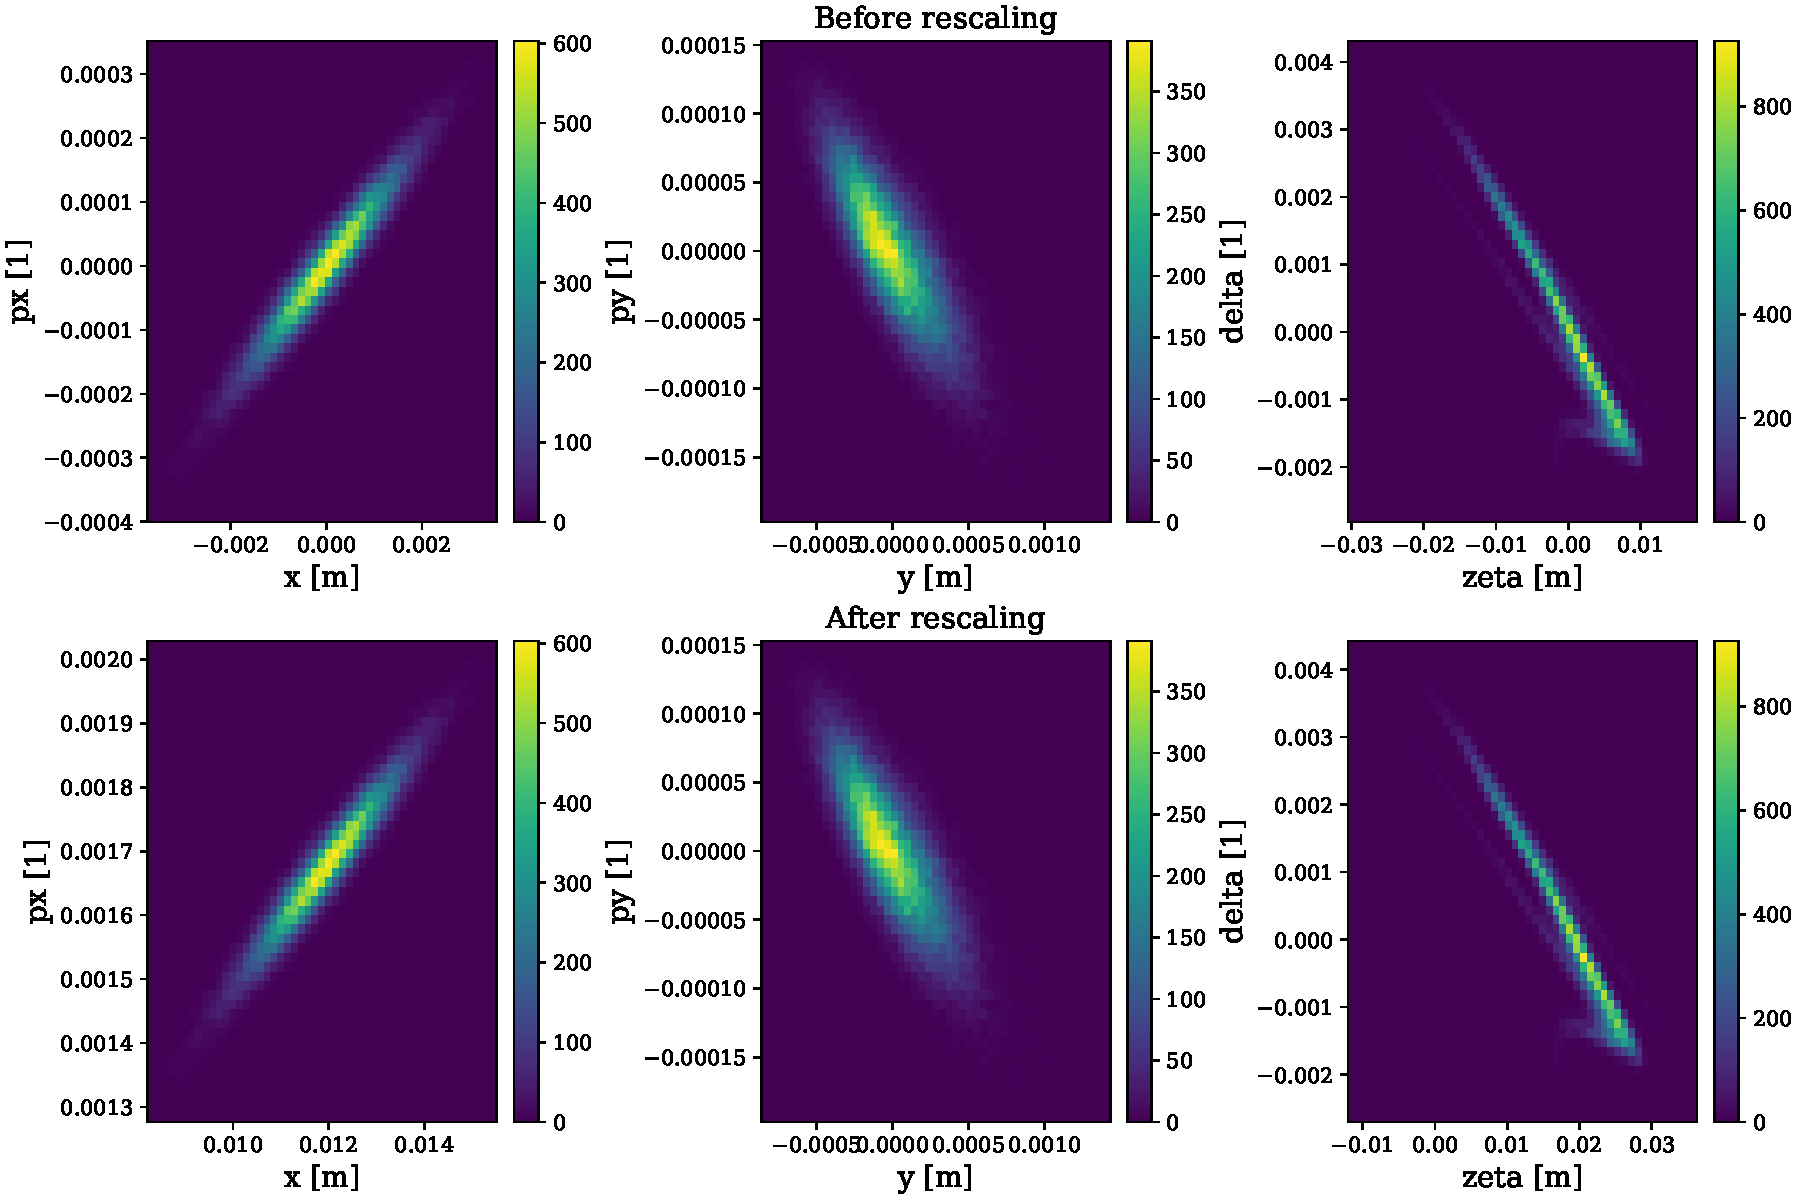
\includegraphics[width=0.8\columnwidth]{Figures/C06_Comparison_with_Simulation/phase_space.pdf}
    \caption{Distribution of the injected particles measured at the end of the beam transport line (top)
    and after rescaling to the target emittances and adding the injection offsets (bottom).}
    \label{fig:phase_space}
\end{figure}


\subsection{Synchrotron radiation}
Xsuite has three options for synchrotron radiation: no radiation, mean radiation and quantum radiation. With mean radiation, each particles loses average radiated energy without fluctuations. With quamtum radiation, the photons are emitted randomly, so the energy loss fluctuate as in the real machine. We used quantum radiation unless stated otherwise. 

\subsection{Beam-beam interaction}
Xsuite offers three models of the beam-beam interaction. The weak-strong 2D model gives a kick based on the Bassetti-Erskine formula neglecting any longitudinal variations of the beam-beam force. The weak-strong 3D model takes into account longitudinal variations of the beam-beam force (hourglass, crossing angle) based on a longitudinal slicing of the beam. The strong-strong model takes into account longitudinal variations of the beam-beam force based on a longitudinal slicing of the both beams, and updated. The computing cost increases in this order. We used the weak-strong 3D model with the HER bunch as the strong beam (Table~\ref{tab:strong_beam}). 

With radiation, the particles are lose energy, and the RF cavities restore it at a shifted synchronous phase. The closed orbit therefore arrives at the interaction point (IP) at at $\zeta = 18.4$~mm instead of $\zeta = 0$. In the machine, the RF timing is set so that the bunches at the same $\zeta$ as the closed orbit. Without this correction, the two bunches would collide at the wrong longitudinal position. 



\begin{table}[htbp]
    \centering
    \caption{Parameters of the strong (HER) bunch in the weak-strong 3D beam-beam model.}
    \label{tab:strong_beam}
    \begin{tabular}{lc}
        \hline
        Beam current / number of bunches & 314.1~mA / 393 \\
        Bunch population & $5.0\times10^{10}$ \\
        Emittance $\varepsilon_x$ / $\varepsilon_y$ & 5.88~nm / 80~pm \\
        $\beta_x^*$ / $\beta_y^*$ & 55~mm / 0.9~mm \\
        Bunch length $\sigma_z$ & 5.1~mm \\
        Half crossing angle & 41.5~mrad \\
        Number of slices & 301 \\
        \hline
    \end{tabular}
\end{table}



\section{Tracking results}
The quality of injection is evaluated with two quantities. The loss map shows where the injected particles are lost during the whole simulation. The survival rate is the fraction of injected particles that remain in the ring, as a function of turn. Figure~\ref{fig:loss_map} shows the loss map. Particles are lost at several vertical and horizontal collimators, but the largest loss is the D06V1 collimator, as in the measurement. 

\begin{figure}[htbp]
    \centering
    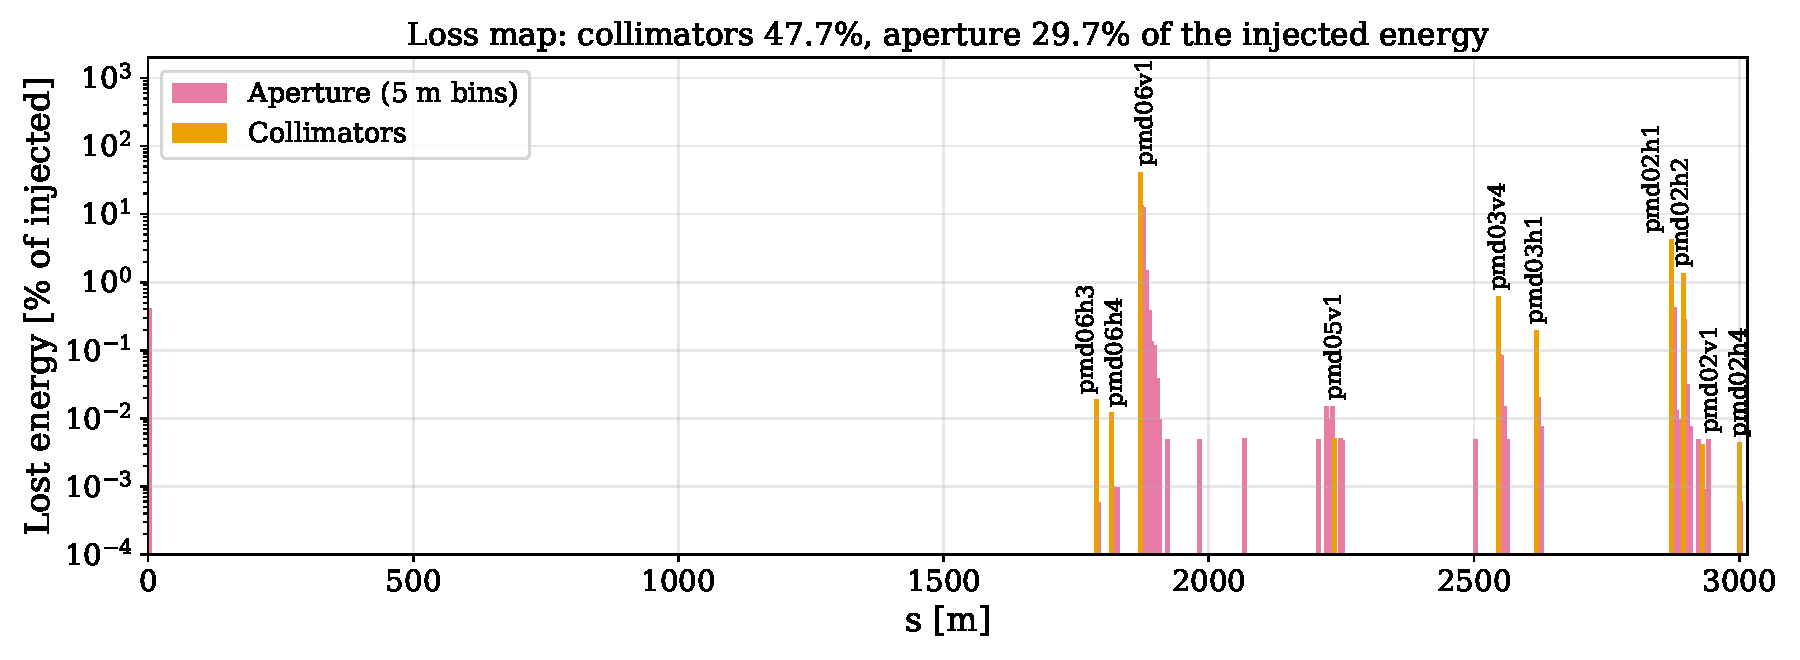
\includegraphics[width=0.8\columnwidth]{Figures/C06_Comparison_with_Simulation/fig_lossmap_quantum_coh.pdf}
    \caption{Loss map of injection simulation (quantum radiation, beam-beam interaction, 2000 turns). The y axis is the energy lost at each collimator (orange) or in 5~m bins of the aperture (pink), in percent of the injected energy. The largest loss is at the D06V1 collimator.}
    \label{fig:loss_map}
\end{figure}


Figure~\ref{fig:survival_rate} shows the survival rate with and without quantum radiation and with and without beam-beam interaction. Radiation increases the survival rate (from 50.8\% to 59.8\% without the beam-beam interaction, and from 15.0\% to 22.3\% with it), because radiation damping reduces the oscillation amplitudes. The beam-beam interaction reduces the survival rate by 36 to 38 percentage points. The measured injection efficiency is about 40--50\%. The simulation without beam-beam interaction (60\%) is above this, and the simulation with it (22\%) is below.
This suggests that the beam-beam effect in the simulation is too strong.



\begin{figure}[htbp]
    \centering
    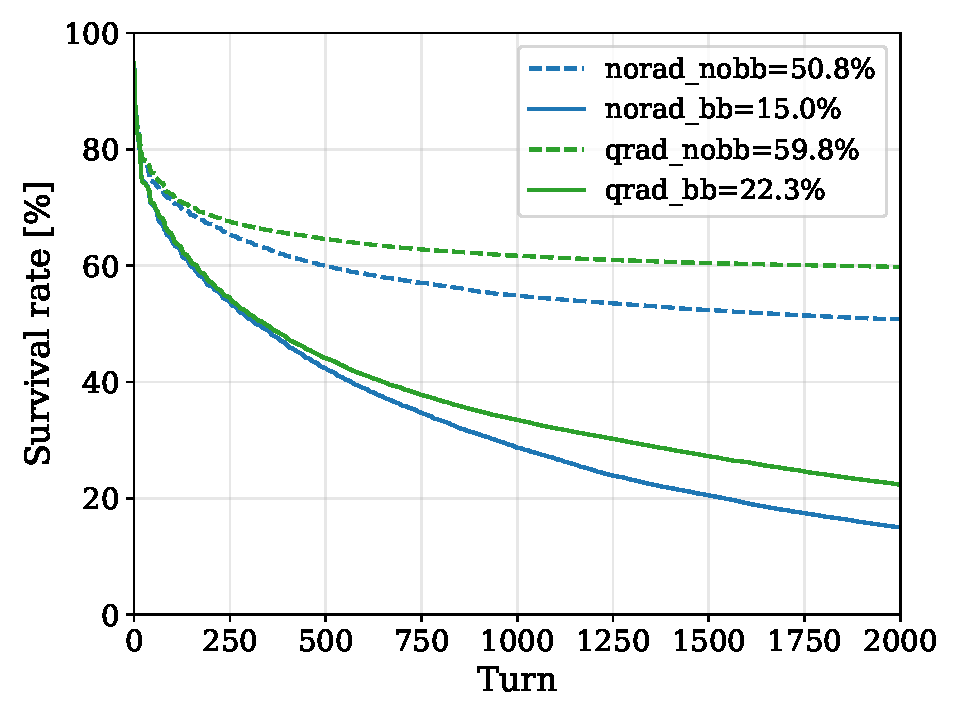
\includegraphics[width=0.6\columnwidth]{Figures/C06_Comparison_with_Simulation/fig_survival_slide.pdf}
    \caption{Survival rate during 2000 turns without radiation (blue) and with quantum radiation (green), with (solid) and without (dashed) the beam-beam interaction.}
    \label{fig:survival_rate}
\end{figure}


\section{Frequency analysis of the loss at D06V1}
As in the measurement, we took the energy loss at the D06V1 in each turn
(Figure~\ref{fig:D06V1_energyFFT}, left) and computed its power spectrum (right). The same window as in the measurement was used: turns 100 to 3999 (3900 turns). Turns after 2000 were not simulated and were set to zero. The signal is sampled once per turn, so a line at fractional tune $q$ appears at $q f_\mathrm{rev}$ or $(1-q) f_\mathrm{rev}$, whichever is below $f_\mathrm{rev}/2 = 49.7$~kHz. The units differ between measurement (V$\cdot$s) and simulation (eV), so only the frequencies, not the heights, can be compared. 

The line near 46~kHz is $(1-\nu_x) f_\mathrm{rev}$, the horizontal betatron tune, as in the measurement.



\begin{figure}[htbp]
    \centering
    \begin{minipage}{0.48\columnwidth}
        \centering
        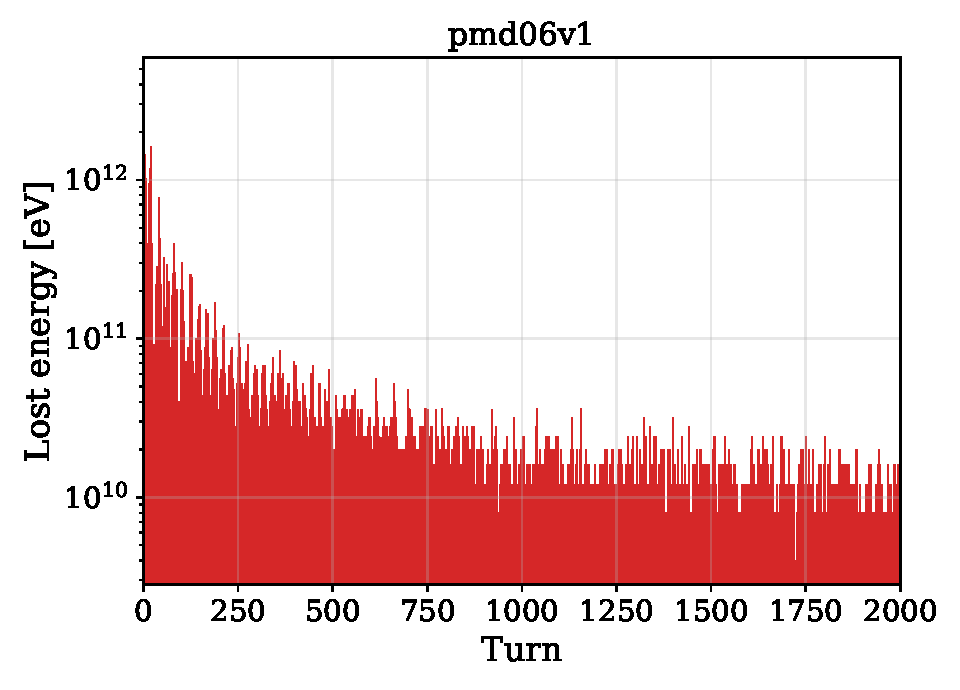
\includegraphics[width=\textwidth]{Figures/C06_Comparison_with_Simulation/fig_lost_energy_quantum_coh_pmd06v1.pdf}
    \end{minipage}
    \hfill
    \begin{minipage}{0.48\columnwidth}
        \centering
        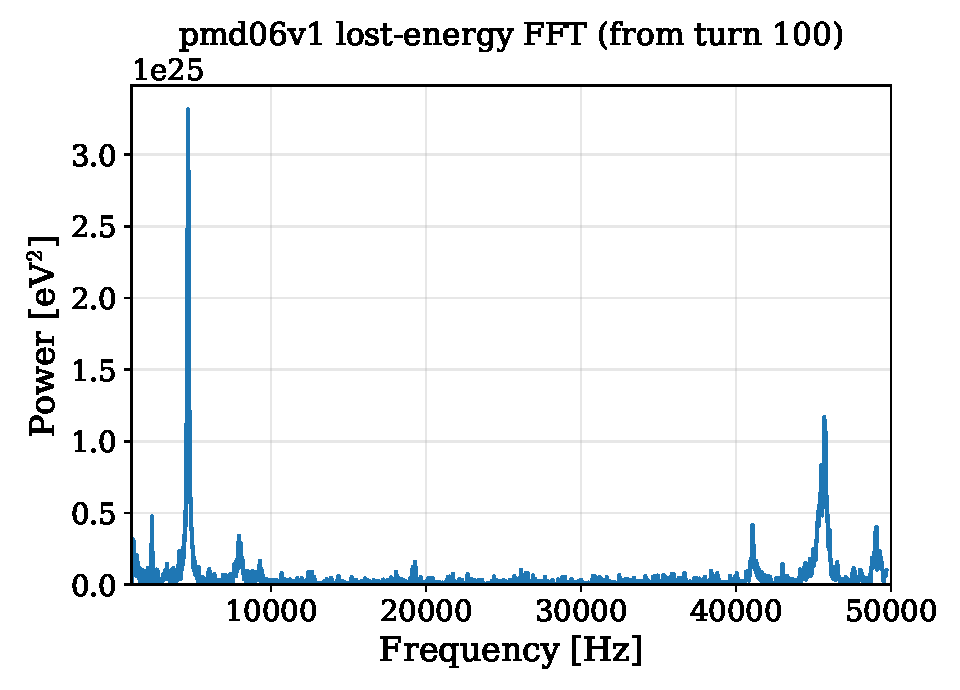
\includegraphics[width=\textwidth]{Figures/C06_Comparison_with_Simulation/fig_fft_energy_quantum_coh_pmd06v1.pdf}
    \end{minipage}
    \caption{Energy lost at the D06V1 collimator in each turn (left) and its power spectrum for turns 100 -- 3999 (right).}
    \label{fig:D06V1_energyFFT}
\end{figure}



\section{Mechanisms of the injection loss}

\subsection{Effect of the horizontal oscillation}
The injected beam oscillates horizontally with a large amplitude, because it is injected with an offset of 11.953~mm. To see how much of the vertical loss this causes, we compared the nominal injection with an injection without the horizontal offset. All other settings are the same (quantum radiation and beam-beam interaction).
Figure~\ref{fig:survival_rate_and_loss_x_osci} shows that the horizontal oscillation reduces the survival rate from 69.2\% to 22.3\%. The energy lost at D06V1 increases from 26.6\% to 69.9\% of the injected energy. Most of the loss at D06V1 is therefore caused by the horizontal oscillation,
although D06V1 is a vertical collimator.


\begin{figure}[htbp]
    \centering
    \begin{minipage}{0.48\columnwidth}
        \centering
        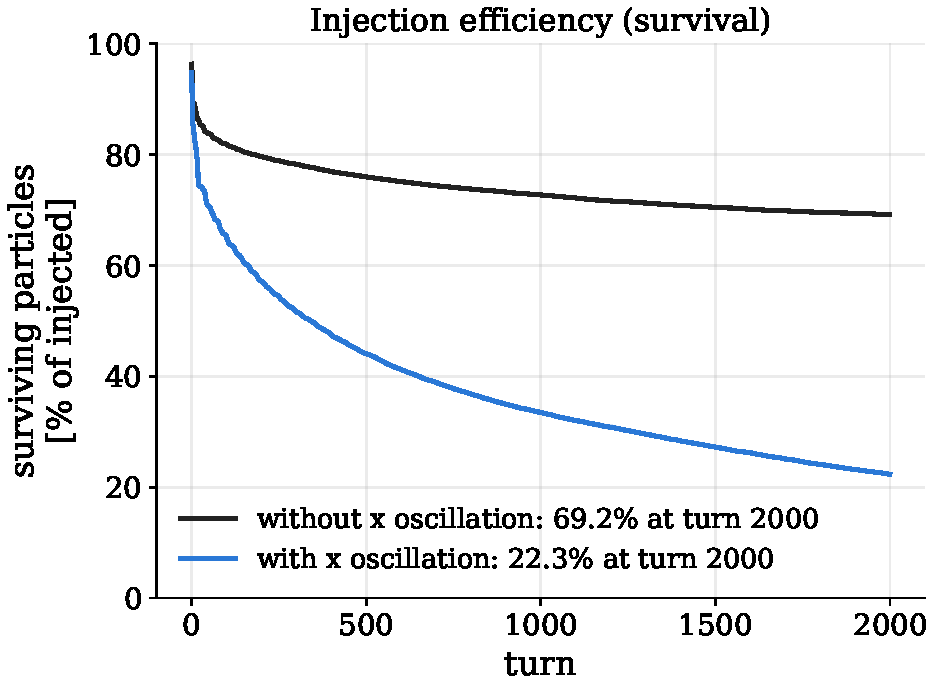
\includegraphics[width=\textwidth]{Figures/C06_Comparison_with_Simulation/A11a_survival.pdf}
    \end{minipage}
    \hfill
    \begin{minipage}{0.48\columnwidth}
        \centering
        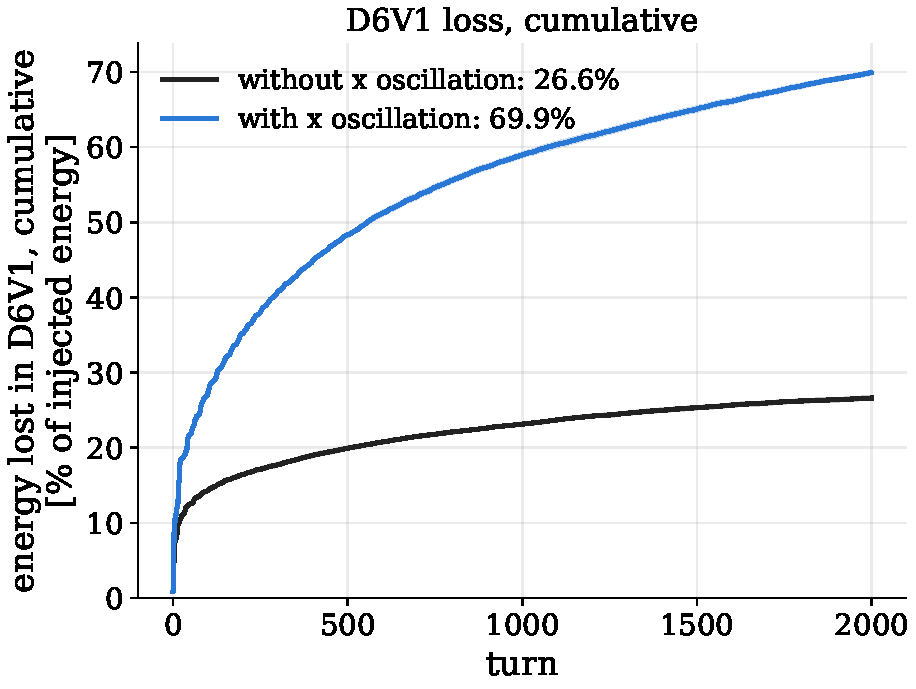
\includegraphics[width=\textwidth]{Figures/C06_Comparison_with_Simulation/A11b_d6v1_loss_cumulative.pdf}
    \end{minipage}
    \caption{Survival rate (left) and cumulative energy loss at the D06V1 collimator (right), with and without the horizontal injection offset.}
    \label{fig:survival_rate_and_loss_x_osci}
\end{figure}


\subsection{Effect of sextupole magnets}
The sextupole magnets connect the horizontal oscillation to the vertical plane. The SuperKEKB LER has 110 sextupole magnets, which correct chromaticity. A particle passing a sextupole with a horizontal offset $x_0$ sees a quadrupole field of strength $k_2 x_0$ (feed-down). For the injected beam, $x_0$ is the centroid oscillation $\langle x \rangle$, so the vertical focusing changes at the horizontal tune. This changes the vertical beta function and the vertical beam size $\sigma_y$ at the horizontal tune, and the loss at the vertical collimator D06V1 follows. 
To test this, we scaled all sextupole magnets together without correcting the chromaticity. To avoid chromatic effects, the initial distribution has no momentum spread ($\delta = 0$). Radiation, beam-beam interaction and collimator were switched off. We computed the spectrum of $\sigma_y$ at D06V1 for turns 10 to 300. Figure~\ref{fig:sigma_y_spectrum} shows that $\sigma_y$ has a clear line at the horizontal tune, jand that this line grows with the sextupole strength. The growth slows down above the nominal strength, because the amplitude of $\langle x \rangle$ itself also depends on the sextupole strength. Normalized by the amplitude of $\langle x \rangle$, the line height is proportional to the sextupole strength (Figure~\ref{fig:sigma_y_spectrum}). Without sextupoles, the line disappears.


\begin{figure}[htbp]
    \centering
    \begin{minipage}{0.48\columnwidth}
        \centering
        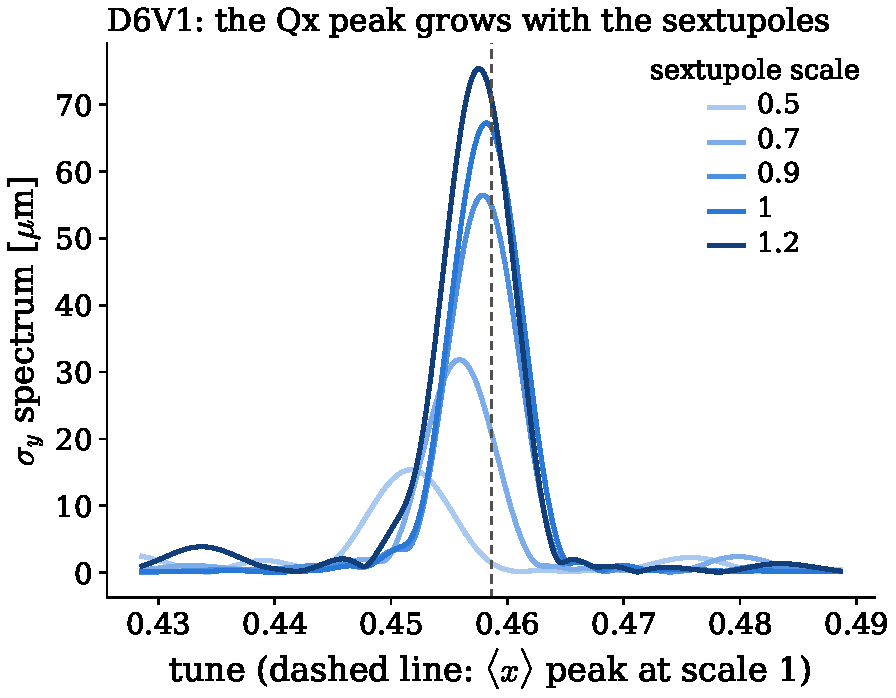
\includegraphics[width=\textwidth]{Figures/C06_Comparison_with_Simulation/A3a_sigma_y_spectrum.pdf}
    \end{minipage}
    \hfill
    \begin{minipage}{0.48\columnwidth}
        \centering
        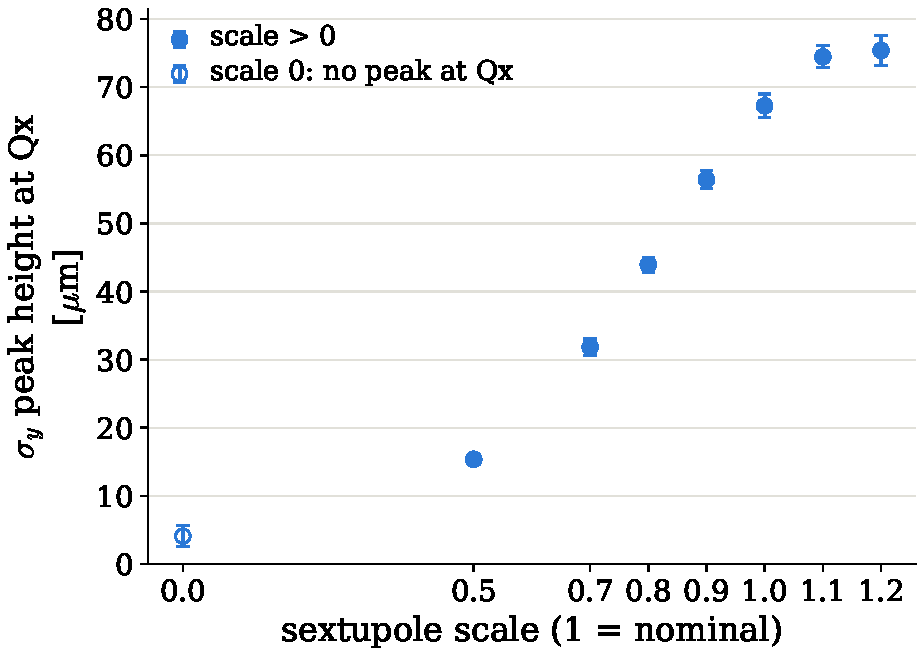
\includegraphics[width=\textwidth]{Figures/C06_Comparison_with_Simulation/A3b_sigma_y_peak_height.pdf}
    \end{minipage}
    \caption{Spectrum of $\sigma_y$ at the D06V1 collimator for several scales of all sextupole magnets (left) and the height of its line at the horizontal tune (right).}
    \label{fig:sigma_y_spectrum}
\end{figure}


\begin{figure}[htbp]
    \centering
    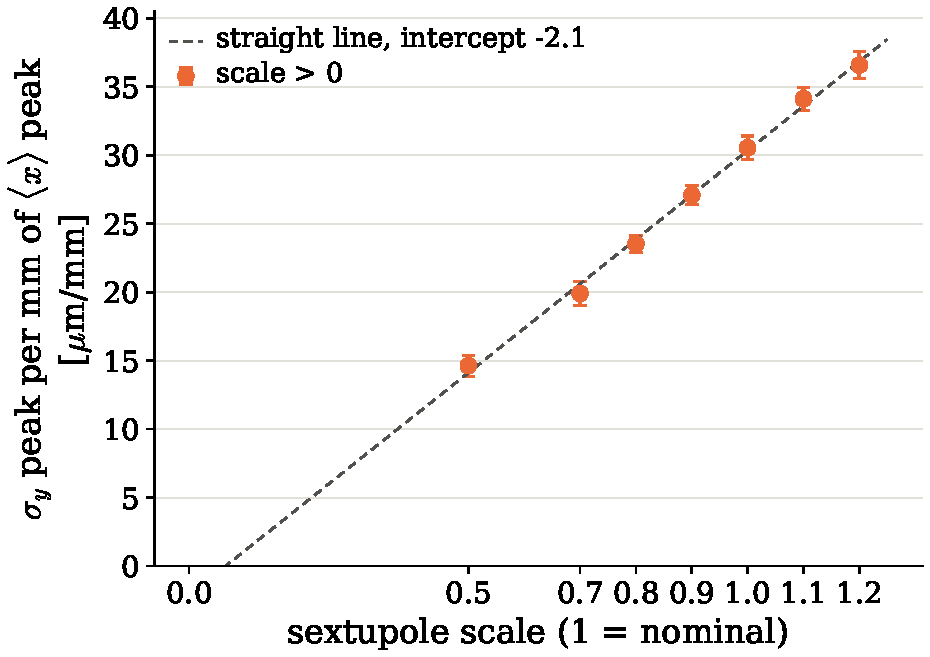
\includegraphics[width=0.6\columnwidth]{Figures/C06_Comparison_with_Simulation/A3c_sigma_y_peak_per_mm.pdf}
    \caption{Height of the $\sigma_y$ line at the horizontal tune per mm of the $\langle x \rangle$ amplitude, against the sextupole scale. The dashed line is a straight-line fit.}
    \label{fig:peak_height_linear}
\end{figure}

Figure~\ref{fig:peak_height_linear} shows that there is linearity between the peak height and sextupole scale. 



The sextupole magnets fall into three groups: 
four vertical-type (SLY) and four horizontal-type (SLX) magnets near the interaction region, and 102 magnets in the arcs. The IR magnets have large strengths $k_2$ and sit where the beta functions are large. To find which group produces the line, we changed the strength of each group by $\pm 10\%$ and took the change of the line height per mm of $\langle x \rangle$ (20000 particles). Figure~\ref{fig:magnet_contribution} shows that the four SLY magnets produce almost al of the line (94\%), the arc magnets 14\%, and the SLX magnets 2\%. The SLY magnets correct the vertical chromaticity and are placed where $\sigma_y$ is large, so their feed-down changes the vertical focusing the most. The shares add up to more than 100\%, because the line height is not exactly proportional ti the sextopole strength (Fig.~\ref{fig:peak_height_linear}).

\begin{figure}[htbp]
    \centering
    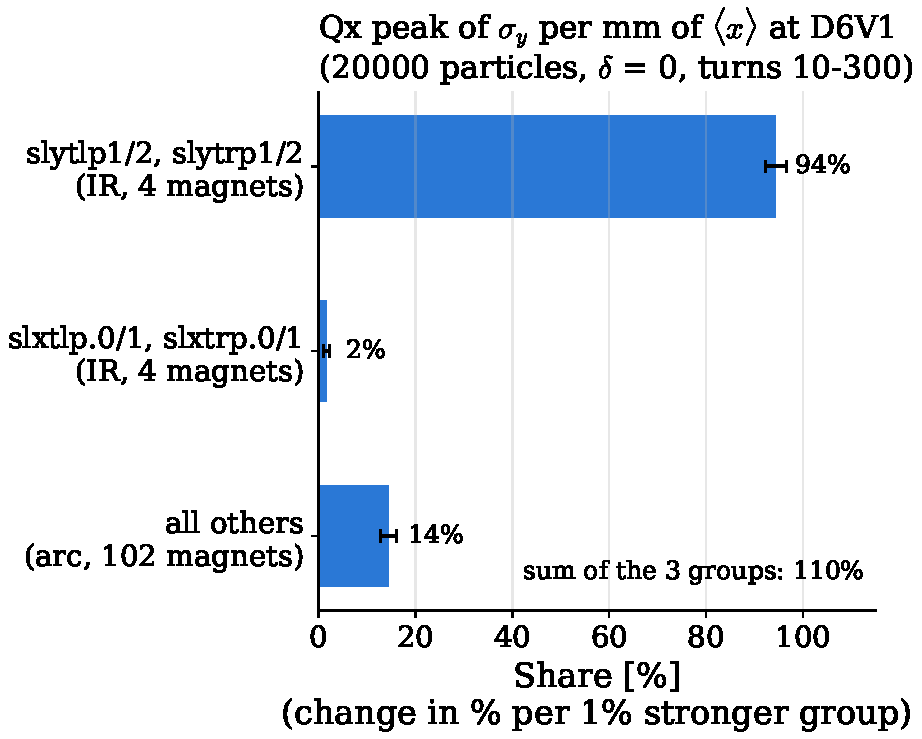
\includegraphics[width=0.6\columnwidth]{Figures/C06_Comparison_with_Simulation/B3_sextupole_group_share.pdf}
    \caption{Share of each sextupole group in the $\sigma_y$ line at the horizontal tune at D06V1: change of the line height (in \%) when the group is made 1\% stronger, from changes of $\pm10\%$.}
    \label{fig:magnet_contribution}
\end{figure}


\section{Summary}
\begin{itemize}
    \item The simulation reproduces the main loss location (D06V1) and the line at the horizontal tune in the loss spectrum. 
    \item The horizontal injection oscillation causes the most loss at D06V1. It sis transferred to the vertical beam size through the feed-down of the sextupole magnets, mainly the four SLY magnets near the IR. 
\end{itemize}













